\chapter{The Visual System}

This chapter covers the neuroscientific context of the thesis. The main part will outline relevant topics concerning the primary visual cortex. For a broader neuroscientific review, we refer the reader to the book Neuroscience: Exploring the brain \citep{bear2020neuroscience}.


\section{The Retina}

The complex process of creating a visual percept in our minds begins in the eye. Firstly, the light passes through the eye’s optical system and projects on the retina, where the first neural response to the light happens. Transformation of the light into a neural response is accomplished by two types of photoreceptors; rods and cones.
Rods do not need a great deal of light to be activated; they are therefore essential for night vision. Cones are complementary, requiring much more light to elicit activity, but their purpose is different; cones provide us with color vision and are smaller, thus providing higher-resolution vision. Three types of cones detect different color spectrum ranges - red, green, and blue.

The visual space projected on the retina and thus perceived by the visual system is called the visual field. It is mainly limited by the eyes’ physiological structure and position in the head. Sometimes we are interested in the area of the visual field where the presence of a stimulus influences the neural activity of a particular cell. This area is called a neuron’s receptive field. The further the cell is in the visual pathway, the larger receptive field it tends to have since it aggregates information from a greater visual field area. The size of an object in our visual field is measured in degrees of visual angle, which describes the distance the object subtends on the retina. As an example, the Moon spans approximately 0.5 degrees of visual angle. One millimeter of retina corresponds to roughly 3.5 degrees of visual angle \citep{bear2020neuroscience}.

After the light is encoded into the neural signal by photoreceptors, the information is sent to bipolar cells and subsequently to ganglion cells. Through horizontal and amacrine cells, ganglion cells obtain aggregated information from the local photoreceptors, allowing them to perform the first nontrivial information processing.

There are two main types of ganglion cells; ON and OFF cells. Their circular receptive field is divided into two regions; a circular center and a surrounding disc. ON and OFF cells are active when they detect a significant luminance difference between the center and the surround. ON cells fire when the center detects proportionally higher luminance than the surround, while OFF cells are active in the opposite situation.

Nevertheless, there are many more types of ganglion cells and other retinal cells, and their functions vary. In conclusion, the retina can detect local changes in contrast or even detect objects’ movement. 

\begin{figure}[H]\centering
	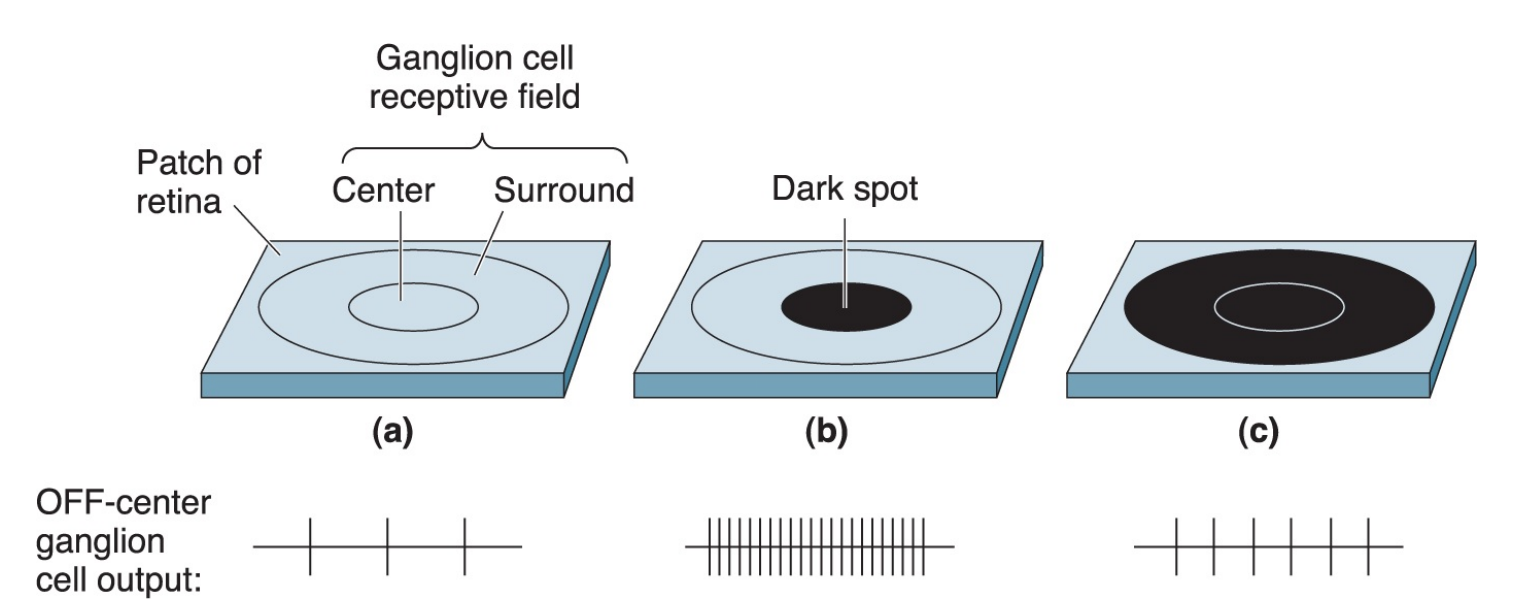
\includegraphics[width=100mm]{../img/on_off_cell.png}
	\caption{Illustration of the OFF cell’s response given different light settings. The highest firing rate of the simple cell is produced when a dark spot surrounded by light is present in the OFF cell’s receptive field. Adapted from \citep{bear2020neuroscience}.}
	\label{img_on_off_cell}
\end{figure}

\section{The Lateral Geniculate Nucleus (LGN)}

When the visual information is encoded and partially processed in the ganglion cell activity, it is sent out of the eye into the brain. The neural signal travels via the optical nerve into the Lateral Geniculate Nucleus (LGN), which is a gateway to the primary visual cortex. LGN is an evolutionarily old brain area located in the dorsal thalamus, and it is connected to numerous different parts of the brain, consequently modulating visual perception. For this reason, recent papers that predict the neural responses in V1 take into account information correlated to other sources of input to LGN \citep{sinz2018stimulus}, for example, locomotion, gaze position, or emotional state of the subject. It is vital to understand that visual processing depends not solely on the visual stimulus but also on other additional information. Without this, neural responses in the V1 can never be entirely explained. 

Right now, research is not focused on this phenomenon. However, if cortical prostheses were to be used in the future, additional data about the implant user would be necessary to acquire the best prosthetic performance.

Visual percept is further processed in LGN in a similar way as it is accomplished in the retina (but with a wider receptive field) and then forwarded to the V1. We must mention that LGN is not a trivial linear gateway to V1. Most of the LGN’s input is paradoxically from the visual cortex. It is unclear what the role of this recurrence is, mainly due to the difficulty of research on this old brain structure lying deep in the middle of the brain, making recording or stimulation experiments targeting this structure challenging. 


\section{The Primary Visual Cortex}

\subsection{The Primary Visual Cortex and Retinotopy}\label{retinotopy}

The first cortical area that is reached by the visual information is the primary visual cortex, also referred to as V1. V1 exhibits the characteristic feature of the central visual system; retinotopy. Retinotopy is a mapping of neural signals from neighboring retinal neurons to neighboring neurons of the LGN and the primary visual cortex. The topology of the visual field is therefore maintained even in the V1.

The striate cortex is about 2\,mm thick. It is morphologically divided into six layers, usually numbered with Roman numbers I to VI, I being the outermost layer and VI the innermost. The most significant portion of the input from the LGN is projected onto layer IV, in particular to sublayer IVC. Many intracortical connections are lateral (parallel to the cortical surface), contributing to combining information from the local neighborhood. Further connections are perpendicular to the cortical surface running through other layers up to layer I, feeding the downstream neurons with input from the same retinal area and maintaining the retinotopic spatial organization in the subsequent layers (Figure~\ref{img_v1_layers}).


\begin{figure}[H]\centering
	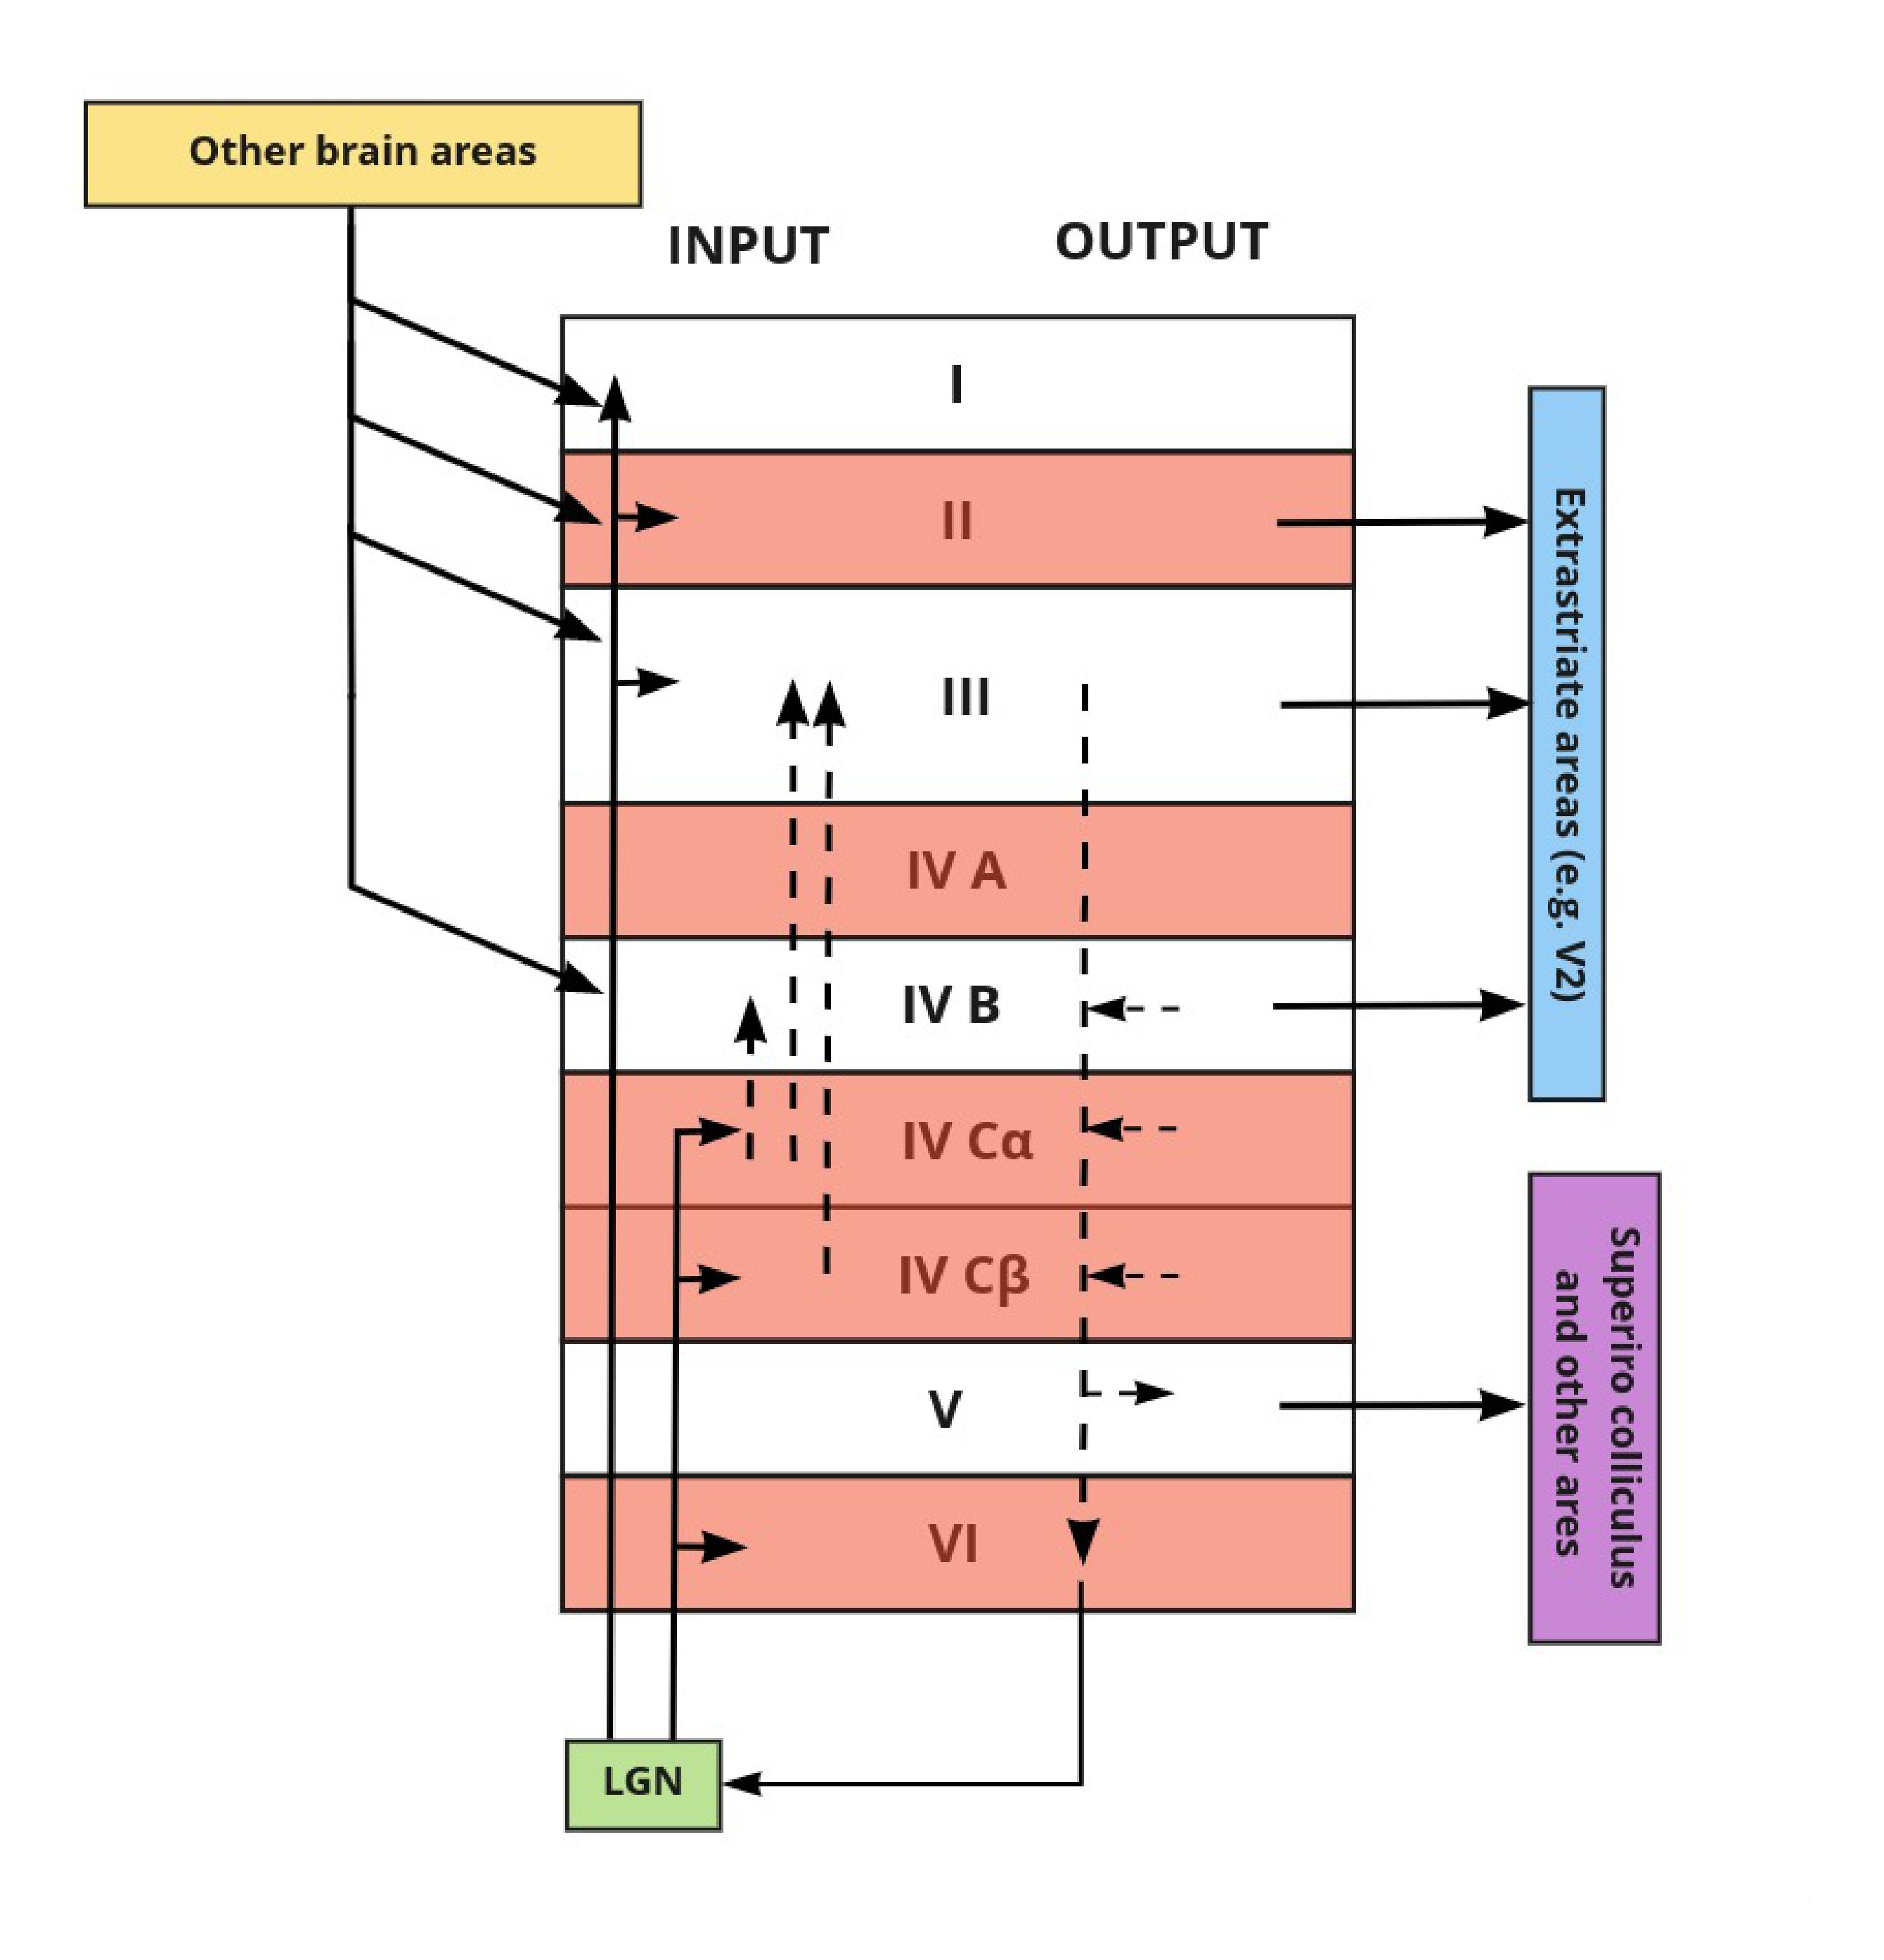
\includegraphics[width=140mm]{../img/final.jpg}
	\caption{A simplified schema of neural input and output of the primary visual cortex. Dashed lines symbolize interconnections between cortical layers. For reasons of clarity, the lateral connections are excluded from this image. Inspired by \citep{bear2020neuroscience} and \citep{kandel2000principles}.}
	\label{img_v1_layers}
\end{figure}


\subsection{Orientation Selectivity}

Besides retinotopy, cells in the previous brain areas on the visual pathway, the retina, and the LGN, have circular receptive fields and some cells manage to detect local changes of luminance in a given point and its surroundings. On the other hand, V1 needs more sophisticated visual patterns for the cells to elicit significant activity. In a famous experiment by Hubel and Wiesel in 1962 \citep{hubel1962receptive}, V1 neurons were found to produce the most significant neural response to elongated bars of light moving across the cell’s receptive field. Furthermore, the cell’s response is selective to the orientation of the bar.

Neurons in the primary visual cortex behave very specifically; many prefer one exact stimulus orientation over the other orientations. If we rotate the stimulus, the response continually decreases until the bar is perpendicular to the preferred orientation, yielding a minimal response (Figure~\ref{img_cat_experiment}). The function describing the response dependency on the orientation of the bar is called the orientation tuning curve. The narrower the tuning curve is, the more orientation selective the cell is said to be.

\begin{figure}[H]\centering
	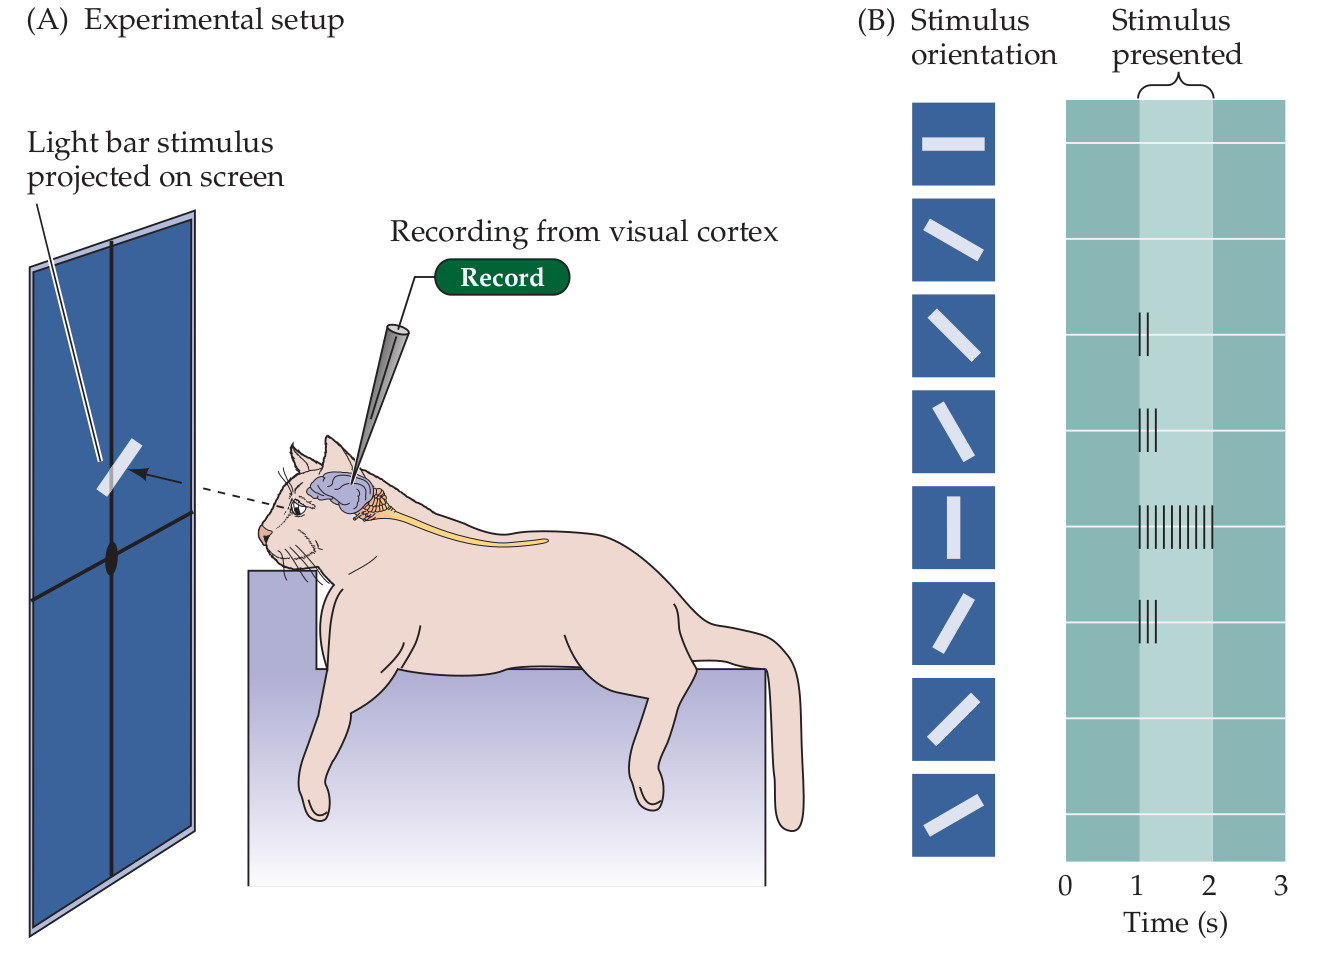
\includegraphics[width=140mm]{../img/cat_experiment.png}
	\caption{Adapted from \citep{purves_2019}.
		(A) An anesthetized cat is equipped with contact lenses to center its gaze on the black dot in the middle of a screen. A white bar of light is presented in the recorded cell’s receptive field in different directions. An extracellular electrode is injected into the cat’s brain to record the particular neuron in the primary visual cortex.
		(B) The cell’s response is dependent on the orientation of the bar. The closer the angle is to the preferred orientation, the higher frequency of spikes is generated by the neuron. 
	}
	\label{img_cat_experiment}
\end{figure}

Orientation preference in the striate cortex also has characteristic spatial properties. As we already know, neurons located on a perpendicular line to the cortical surface process information from the exact location on the retina and the corresponding location in the visual field. Similarly, these neurons also have the same preferred orientation. Moreover, in higher mammals, neighboring cells in the tangential direction to the cortical surface possess similar orientation preferences, which is not the case in rodents \citep{van2005orientation}, \citep{bednar2016cortical}. If we inserted an electrode tangentially into the higher-mammalian V1 tissue, we would observe the orientation preference to periodically and continuously change (Figure~\ref{img_periodic_orientation}).


\begin{figure}[H]\centering
	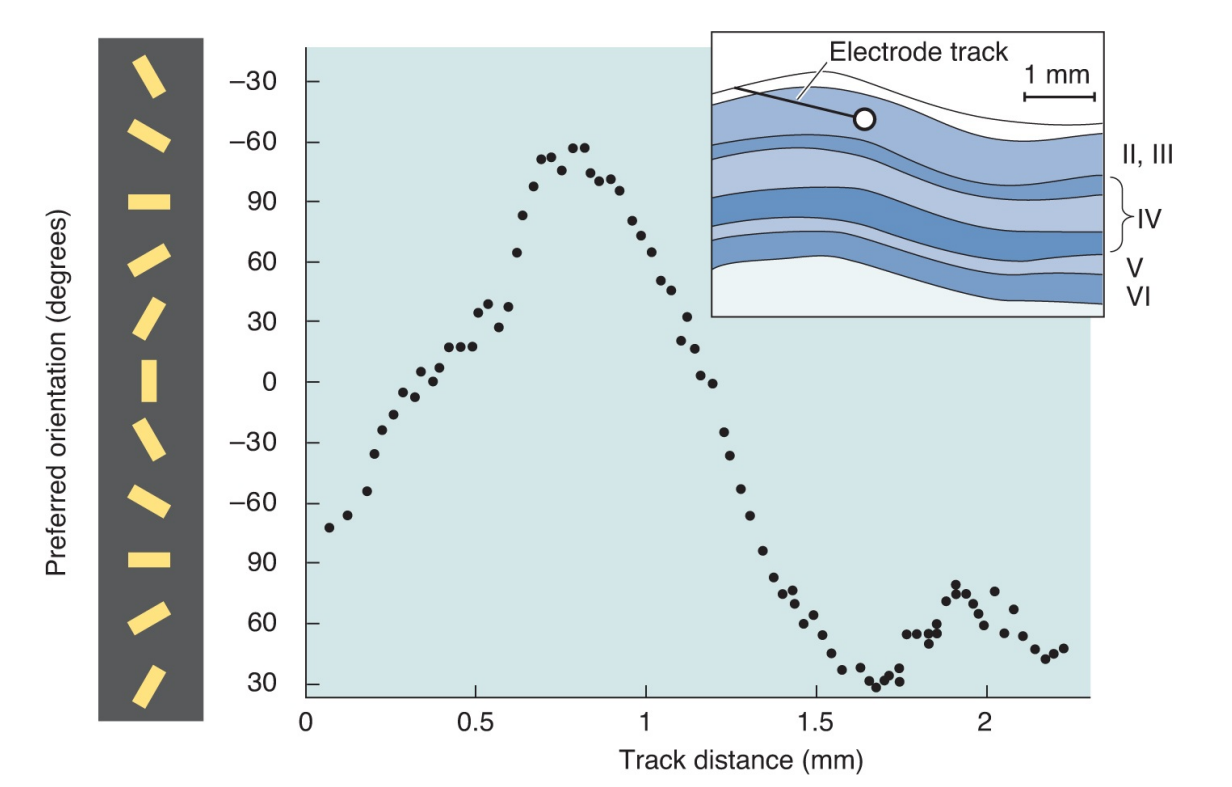
\includegraphics[width=140mm]{../img/tangengal_electrode_orientation.png}
	\caption{Since tangentially neighboring cells have similar orientation preferences, tangental insertion of a recording electrode into the striate cortex of higher mammals records a continuous change of the orientation preference. Moreover, this change is periodic. Adapted from \citep{bear2020neuroscience}.}
	\label{img_periodic_orientation}
\end{figure}


Consequently, the primary visual cortex can be functionally organized into orientation columns, columns of cells parallel to V1, comprising neighboring neurons with very similar orientation selectivity (Figure~\ref{ori_columns}).


\begin{figure}[H]\centering
	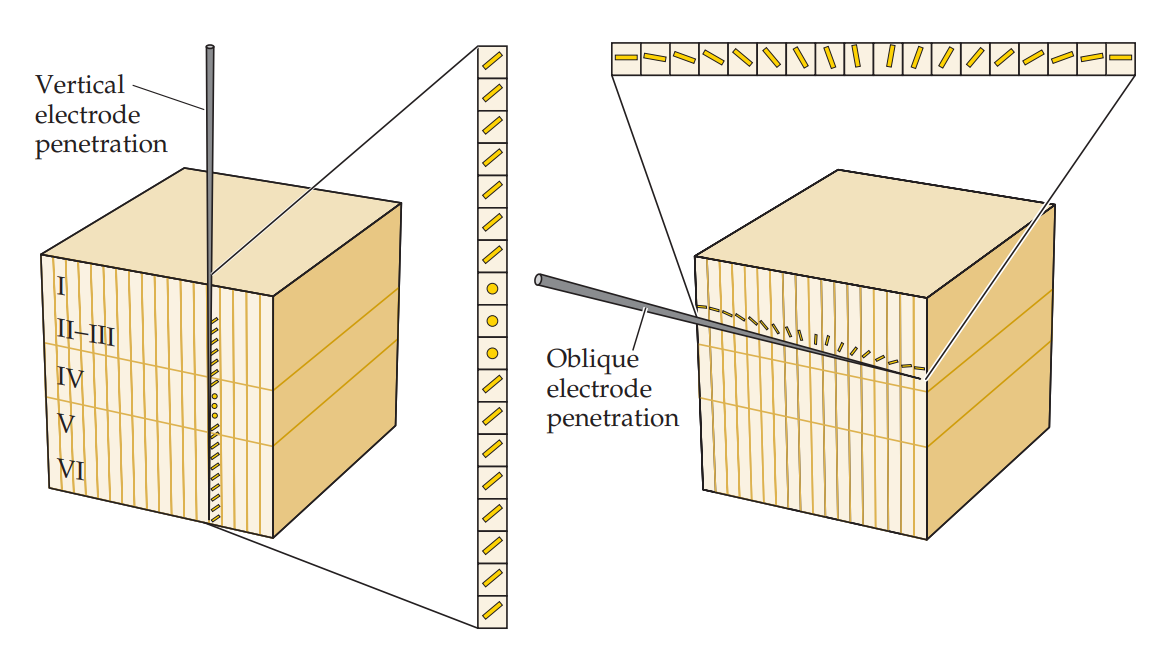
\includegraphics[width=140mm]{../img/orientation_columns.png}
	\caption{Orientation columns in monkey V1. As a measurement from the electrodes suggests, when the electrode is inserted vertically (perpendicularly to the cortex), the preferred orientation does not change. If inserted tangentially (obliquely) to the cortex, the preferred orientation shifts continually and periodically. Adapted from \citep{purves_2019}.}
	\label{ori_columns}
\end{figure}

It is possible to reconstruct and visualize the preferred orientation in the striate cortex \citep{smith2018distributed}. The result is called an \emph{orientation map}, and it is essential to note that it differs from subject to subject (Figure~\ref{ori_map_first}). In higher mammals, the neighboring regions of this map, where the preferred orientations of neurons are similar, are called \emph{orientation domains}.

\begin{figure}[H]\centering
	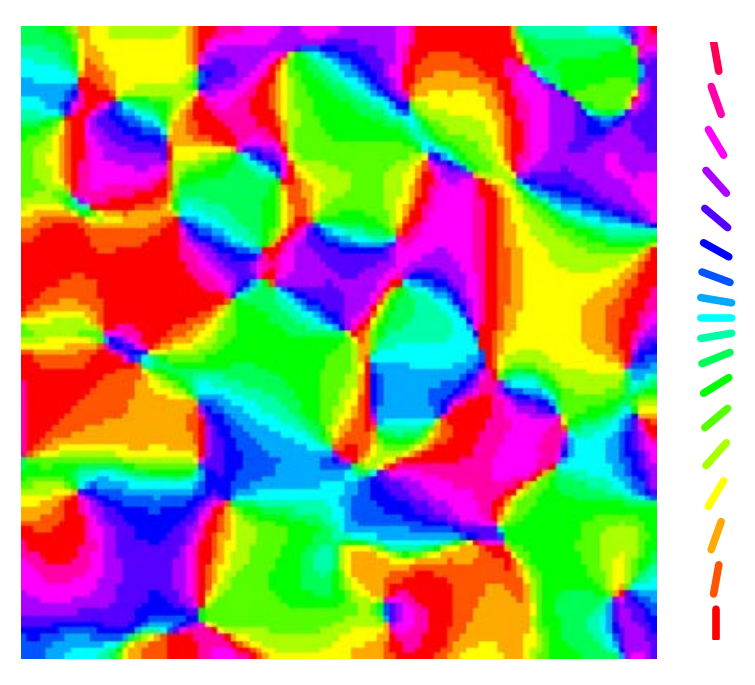
\includegraphics[width=80mm]{../img/orientation_map.png}
	\caption{Visualization of orientation preference map. Each color corresponds to a particular angle, as shown on the right. Adapted from \citep{lam2005self}.}
	\label{ori_map_first}
\end{figure}


\subsection{Simple and Complex Cells}

Two main functional types of cells are present in the striate cortex. The first type, simple cells, detect oriented bars on an exact position in their receptive field, as explained in the previous section. In their receptive field, some areas are either excitatory or inhibitory, resulting from their response being a linear combination of ON and OFF cells on the simple cell’s input. Their receptive fields behave as a Gabor filter and are therefore commonly modeled this way.

On the other hand, complex cells’ output cannot be modeled simply as a linear transformation of the visual input. Their receptive field is not divided into strictly excitatory or inhibitory regions. Compared to simple cells, complex cells are invariant to the stimulus position in the receptive field. Still, they are orientation selective. 








